\section{Dynamic Switching Visualization} \label{switching-visualization}
The configuration switching happens during both phases of the READEX methodology. 
During DTA, PTF runs experiments with different configurations to find the optimal configuration for each rts in the application, which are then stored in the tuning model. During RAT, RRL applies the optimal configuration from the tuning model for each rts during the application run. Both stages require configuration switching during the application run.

To enable the user to visualize the configuration switching for each region during DTA and during a production run, a switching visualization module is included in the RRL. 
The visualization module is implemented as a Score-P Metric Plugin. The metric plugin uses the Metric Plugin Interface provided in Score-P \cite{Schoene2017}. The user can select any of the hardware, software and application tuning parameters to visualize the switching pattern. The tuning parameters selection is configurable and the user can specify if all the tuning parameters or a subset has to be recorded. Each of the tuning parameters is then added as a metric and recorded in a trace in the \textit{OTF2} format \cite{Ilsche-Cstate} by Score-P. The trace can be visualized in the Vampir \cite{BHJR:10:VampirOverview}. 
 
Figure~\ref{fig:switch_visualization} illustrates the switching of the CPU frequency and uncore frequency performed by RRL while tuning CPU frequency and uncore frequency for the Blasbench benchmark. The top timeline shows the call stack of application regions. Below that we see the core frequency which changes between 1.5 and 1.5 GHz. Finally the changes of the uncore frequency is shown following the optimal settings of the different regions.

\begin{figure}[!t]
\centering
%\includegraphics[trim={7cm 2cm 5.5cm 2cm},clip,width=3in]{readex-approach}
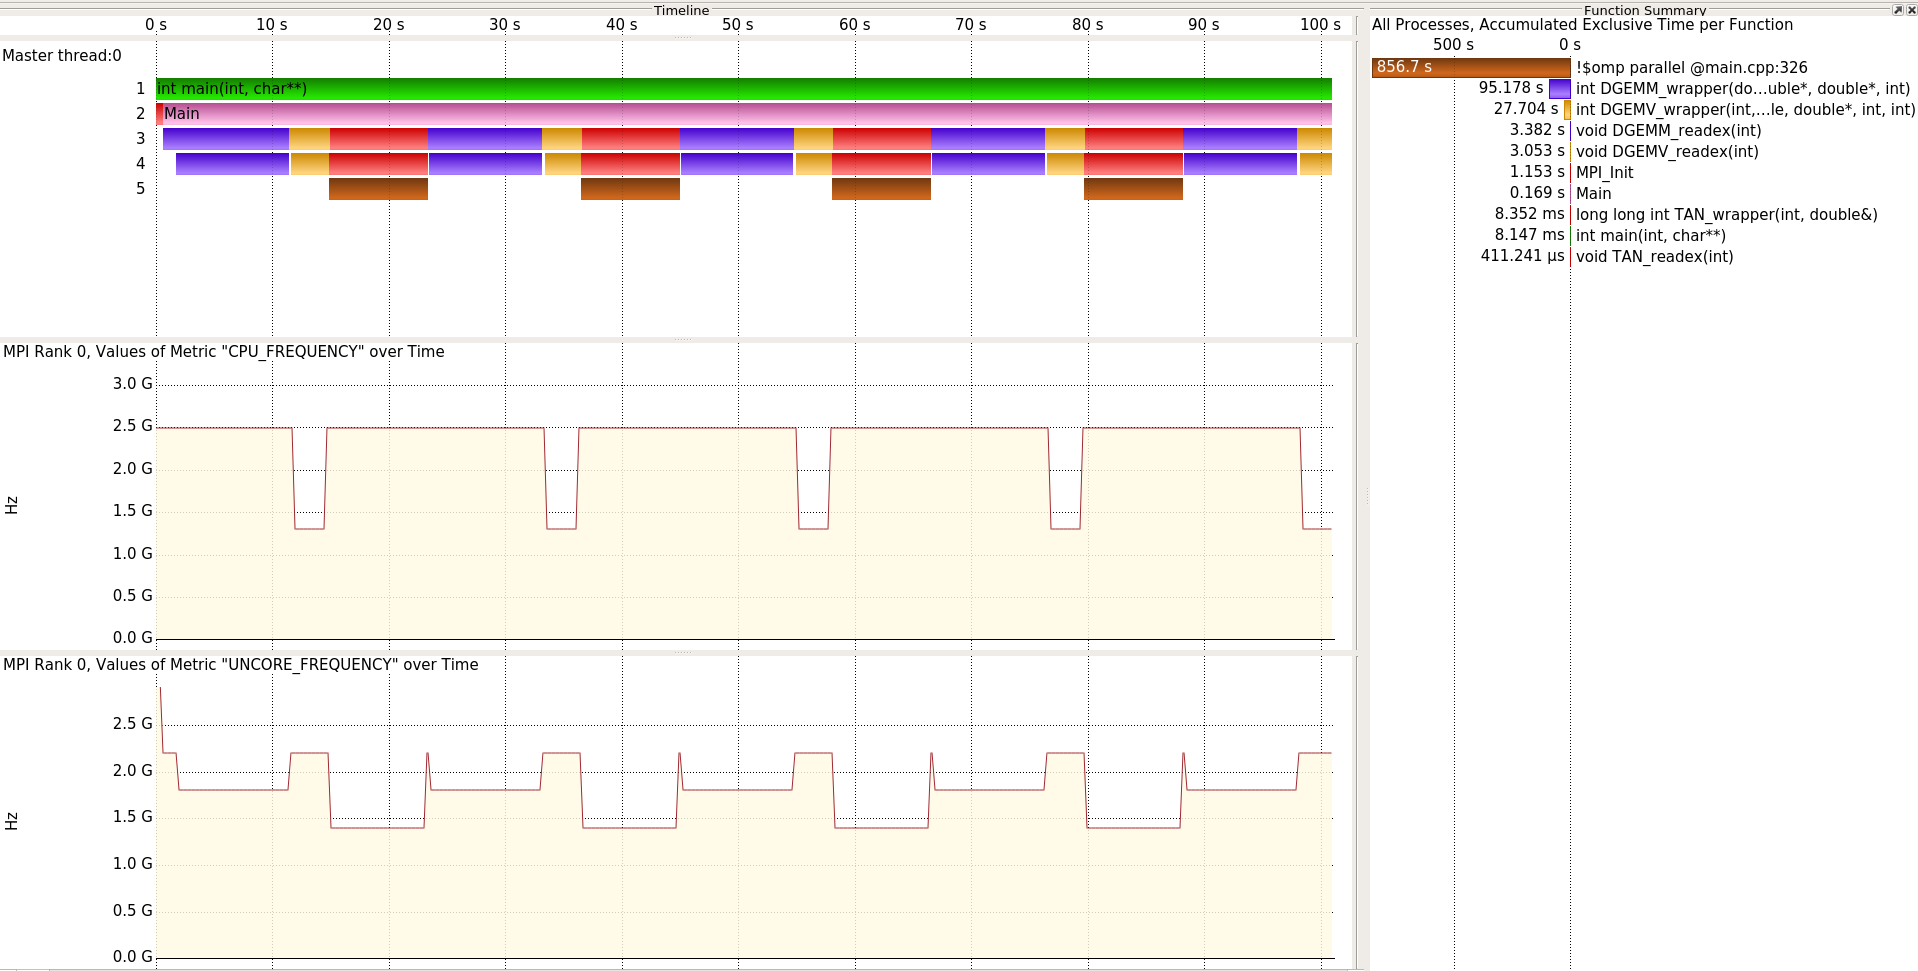
\includegraphics[width=.95\columnwidth]{figures/visualization_trace.png}
\caption{{CPU\_FREQUENCY} and {UNCORE\_FREQUENCY} switchings during Blasbench runtime tuning}
\label{fig:switch_visualization}
\end{figure}

 